\documentclass[]{article}
\usepackage{lmodern}
\usepackage{amssymb,amsmath}
\usepackage{ifxetex,ifluatex}
\usepackage{fixltx2e} % provides \textsubscript
\ifnum 0\ifxetex 1\fi\ifluatex 1\fi=0 % if pdftex
  \usepackage[T1]{fontenc}
  \usepackage[utf8]{inputenc}
\else % if luatex or xelatex
  \ifxetex
    \usepackage{mathspec}
  \else
    \usepackage{fontspec}
  \fi
  \defaultfontfeatures{Ligatures=TeX,Scale=MatchLowercase}
\fi
% use upquote if available, for straight quotes in verbatim environments
\IfFileExists{upquote.sty}{\usepackage{upquote}}{}
% use microtype if available
\IfFileExists{microtype.sty}{%
\usepackage{microtype}
\UseMicrotypeSet[protrusion]{basicmath} % disable protrusion for tt fonts
}{}
\usepackage[margin=1in]{geometry}
\usepackage{hyperref}
\hypersetup{unicode=true,
            pdftitle={Analysis of electric vehicle usage patterns in New Zealand},
            pdfauthor={Rafferty Parker and Ben Anderson (University of Otago)},
            pdfborder={0 0 0},
            breaklinks=true}
\urlstyle{same}  % don't use monospace font for urls
\usepackage{longtable,booktabs}
\usepackage{graphicx,grffile}
\makeatletter
\def\maxwidth{\ifdim\Gin@nat@width>\linewidth\linewidth\else\Gin@nat@width\fi}
\def\maxheight{\ifdim\Gin@nat@height>\textheight\textheight\else\Gin@nat@height\fi}
\makeatother
% Scale images if necessary, so that they will not overflow the page
% margins by default, and it is still possible to overwrite the defaults
% using explicit options in \includegraphics[width, height, ...]{}
\setkeys{Gin}{width=\maxwidth,height=\maxheight,keepaspectratio}
\IfFileExists{parskip.sty}{%
\usepackage{parskip}
}{% else
\setlength{\parindent}{0pt}
\setlength{\parskip}{6pt plus 2pt minus 1pt}
}
\setlength{\emergencystretch}{3em}  % prevent overfull lines
\providecommand{\tightlist}{%
  \setlength{\itemsep}{0pt}\setlength{\parskip}{0pt}}
\setcounter{secnumdepth}{5}
% Redefines (sub)paragraphs to behave more like sections
\ifx\paragraph\undefined\else
\let\oldparagraph\paragraph
\renewcommand{\paragraph}[1]{\oldparagraph{#1}\mbox{}}
\fi
\ifx\subparagraph\undefined\else
\let\oldsubparagraph\subparagraph
\renewcommand{\subparagraph}[1]{\oldsubparagraph{#1}\mbox{}}
\fi

%%% Use protect on footnotes to avoid problems with footnotes in titles
\let\rmarkdownfootnote\footnote%
\def\footnote{\protect\rmarkdownfootnote}

%%% Change title format to be more compact
\usepackage{titling}

% Create subtitle command for use in maketitle
\newcommand{\subtitle}[1]{
  \posttitle{
    \begin{center}\large#1\end{center}
    }
}

\setlength{\droptitle}{-2em}

  \title{Analysis of electric vehicle usage patterns in New Zealand}
    \pretitle{\vspace{\droptitle}\centering\huge}
  \posttitle{\par}
  \subtitle{Statistical Report}
  \author{Rafferty Parker and Ben Anderson (University of Otago)}
    \preauthor{\centering\large\emph}
  \postauthor{\par}
      \predate{\centering\large\emph}
  \postdate{\par}
    \date{Last run at: 2019-02-04 10:40:58}

\usepackage{booktabs}
\usepackage{longtable}
\usepackage{array}
\usepackage{multirow}
\usepackage{wrapfig}
\usepackage{float}
\usepackage{colortbl}
\usepackage{pdflscape}
\usepackage{tabu}
\usepackage{threeparttable}
\usepackage{threeparttablex}
\usepackage[normalem]{ulem}
\usepackage{makecell}
\usepackage{xcolor}

\begin{document}
\maketitle

{
\setcounter{tocdepth}{2}
\tableofcontents
}
\section{Introduction}\label{introduction}

The New Zealand government has set a target of increasing the number of
EVs in New Zealand to 64,000 by 2021. High penetration of EVs would
cause EV recharging to contribute a substantial portion of total
electricity load. A report prepared for lines companies Orion, Powerco
and Unison by Concept Consulting Group entitled ``Driving change -
Issues and options to maximise the opportunities from large-scale
electric vehicle uptake in New Zealand'' predicts that if all current
light private vehicles were electric, annual residential electricity
consumption would increase by approximately 30\%, whereas if all
vehicles including trucks were electric, this would increase the total
electricity consumption of New Zealand by approximately
41\%{[}concept\_2018{]}.

New Zealand's total electricity demand varies throughout the day, with
weekdays in particular having two distinct ``peaks''; one in the
morning, and one in the evening. Providing the electicity to meet these
demand peaks is a costly and inefficient process. Concurrent electric
vehicle (EV) charging, especially in the early evening when many
motorists return home, would have the potential to negatively impact the
operation of the grid through drastically increasing peak loads
{[}Azadfar2015{]}, leading to an increased cost of electricity due to
the requirement of expensive upgrades to the electricity
grid{[}@stephenson\_smart\_2017{]}.

This report hopes to provide further insight into the potential effects
on the New Zealand electricity grid that may occur with a dramatic
increase in EVs, so that these may be planned for and mitigated. It is
based on and inspired by the
\href{https://assets.publishing.service.gov.uk/government/uploads/system/uploads/attachment_data/file/764270/electric-chargepoint-analysis-2017-domestics.pdf}{UK
DoT statistical report 2018}.

\section{Data information}\label{data}

\subsection{Background}\label{background}

The data used has been provided by ``Flip the Fleet'', a community
organisation that hopes to increase uptake of electric vehicles in New
Zealand. Flip the Fleet have been collecting data on electric vehicle
usage patterns, collected using Exact IOT Limited's
\href{https://flipthefleet.org/ev-black-box/}{blackbox recorder}, a
small electronic device that connects to the vehicle's internal computer
and sends detailed data about the battery health, consumption, speed,
etc.

The data used consisted of 1291881 data points from 44 vehicles over 8
months (April 2018 - January 2019). The recorder provided measurements
at 1 minute frequency of charging behaviour and battery charge state.

Due to privacy considerations, the data is not publically available.

\subsection{Initial cleaning}\label{initial-cleaning}

There were 6 vehicles in the data provided that had no recorded charging
occur. These were immediately discarded.

Some instances of charging power greater than 120kW were recorded. These
were considered anomolies and discarded, as these exceed the capacity of
the highest charging stations available in New
Zealand{[}@concept2018{]}.

Instances of battery state of charge being greater than 100\% or less
than 0\% were also discarded.

\subsection{Definitions and
preparation}\label{definitions-and-preparation}

Charging data has been broadly seperated into two seperate catagories,
``standard'' and ``fast''. Standard charging is when the charger is
reading less than 7kW - this is considered the upper limit of what can
be obtained from a standard home charging scenario without an expensive
wiring upgrade{[}@concept2018{]}. Fast charging is all charging above
7kW, and would likely occur at designated and purpose-built fast
charging stations.

The data was also catagorised according to whether it was a weekday or
not. This allows analysis to occur of differing charging patterns
between weekdays and weekends, allowing for further accuracy in
determining the effects of electric vehicles on grid peaks.

In order to determine charging durations, rows were initially flagged as
``charging begins'' if the charging power was greater than zero and the
previous and following row's charging power were (respectively) equal to
zero and greater than zero. Similarly, rows were flagged as ``charge
ends'' if the charging power was greater than zero and the previous and
following row's charging power were (respectively) greater than zero and
equal to zero.

Using this method we obtained 7376 instances of charge beginning, and
7385 instances of charge ending. The additional 9 instances of the
charge ending than there are of the charge beginning may be due to the
first instance of data collection occurring during mid-charge for some
vehicles.

If we assume that the first non-zero charge observation is the `start'
and the last non-zero charge observation within the vehicle id is the
`end' we can calculate the duration between the two. This assumes there
is no missing data.

Figure \ref{fig:durationHist} shows the overall distribution of all
charging sequences. Clearly there are very small and a few very large
values for Standard Charges, but this is not the case for Fast charges.

\begin{figure}
\centering
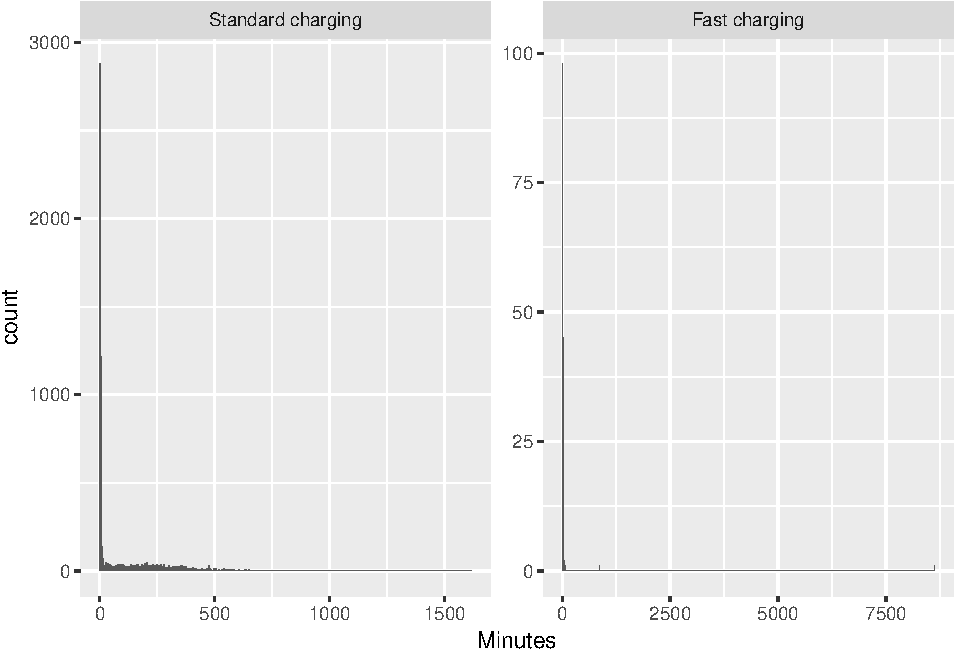
\includegraphics{EVBB_report_files/figure-latex/durationHist-1.pdf}
\caption{\label{fig:durationHist}Duration of charging sequences}
\end{figure}

Table \ref{tab:durationDescTable} shows the overall distributions and
indicates the extent to which the means are skewed by the very small and
a few very large values shown in Figure \ref{fig:durationHist}.

\begin{table}[t]

\caption{\label{tab:durationDescTable}Duration of all charge sequences by charge type (minutes)}
\centering
\begin{tabular}{l|r|r|r|r|r}
\hline
chargeType & N & mean & median & min & max\\
\hline
Standard charging & 6983 & 101.24 & 3.72 & 0.27 & 1616.72\\
\hline
Fast charging & 392 & 38.00 & 12.48 & 0.32 & 8621.00\\
\hline
\end{tabular}
\end{table}

Figure \ref{fig:shortDuration} shows the distribution of very short
charging sequences. As we can see these appear to be generally less than
8 minutes in length for Standard Charges.

\begin{figure}
\centering
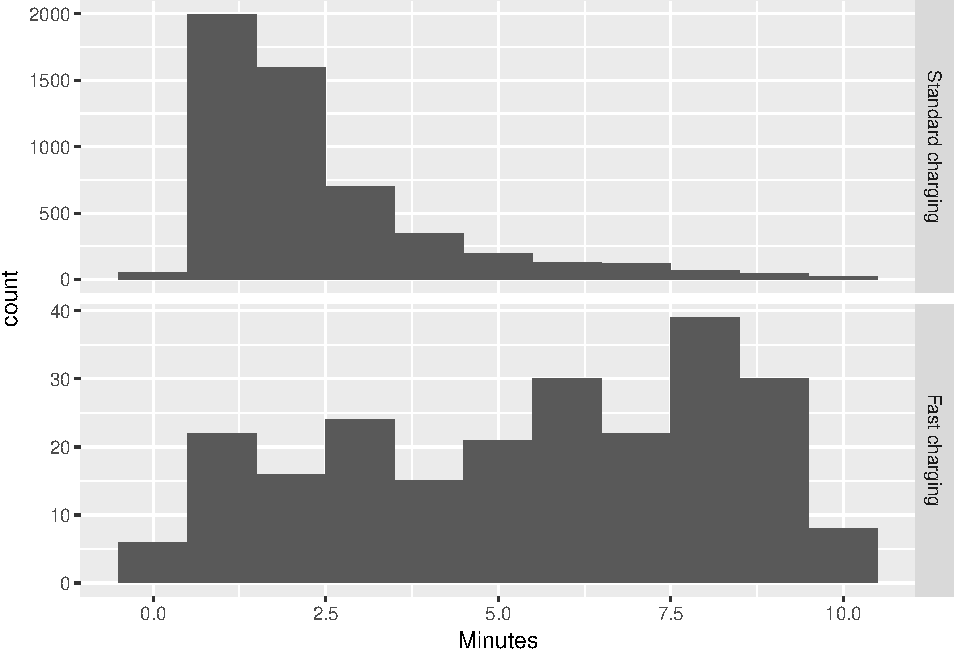
\includegraphics{EVBB_report_files/figure-latex/shortDuration-1.pdf}
\caption{\label{fig:shortDuration}Duration of charging sequences \textless{}
10 minutes}
\end{figure}

Table \ref{tab:durationDescTableReduced} shows the same descriptive
statistics but for all sequences of greater than 8 minute duration. Now
we can see that the mean and median durations for Standard Charge
sequences are closer to one another.

\begin{table}[t]

\caption{\label{tab:durationDescTableReduced}Duration of charge sequences > 8 minutes by charge type (minutes, )}
\centering
\begin{tabular}{l|r|r|r|r|r}
\hline
chargeType & N & mean & median & min & max\\
\hline
Standard charging & 2860 & 244.01 & 208.65 & 8.02 & 1616.72\\
\hline
Fast charging & 279 & 51.61 & 15.73 & 8.05 & 8621.00\\
\hline
\end{tabular}
\end{table}

Manual inspection of the data showed that these short-duration charging
``events'' generally occurred near the end of a longer-duration charging
event. It appeared that once the vehicle had reached its highest state
of charge, charging would intermittantly stop and start again, often at
low power (\textless{} 1kW). This is likely due to the behaviour of the
charger once the battery was almost full. As these can not be considered
truly independent charging events, they have been removed from the data
for the rest of the analysis.

In addition to the myriad ``small'' charging duration values, two very
large charging durations (longer than 100 hours) were calculated. As
even a very high capacity vehicle using the slowest standard charger
would not take this long to charge from empty, these were assumed to be
anomalies and were discarded.

Figure \ref{fig:longDuration} shows the distribution of charging
sequences with the excessively long or short events removed. As we can
see these appear to be generally less than 3 hours in length for
Standard Charges.

All further duration-related analysis is conducted with these
excessively long or short events removed from the data.

\begin{figure}
\centering
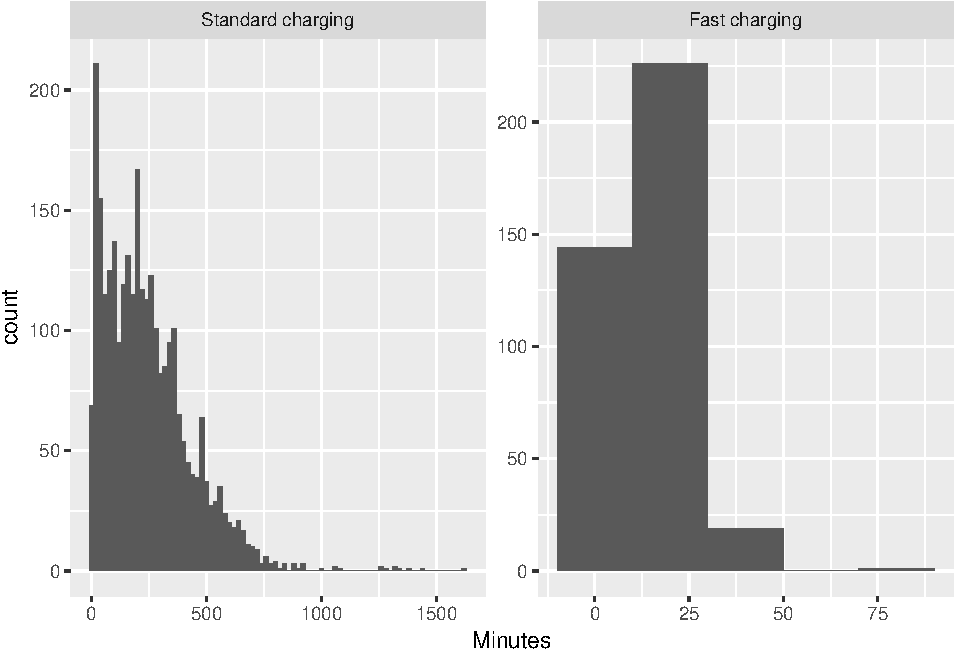
\includegraphics{EVBB_report_files/figure-latex/longDuration-1.pdf}
\caption{\label{fig:longDuration}Duration of charging sequences
\textgreater{} 8 minutes}
\end{figure}

\section{Key Findings:}\label{key-findings}

\begin{itemize}
\tightlist
\item
  \emph{Power supplied}: The median power supplied during a standard
  charging was 1.78 kW. The mean was slightly higher at 2.12 kW. Fast
  charging observations had a median of 30.84 kW (mean = 30.68);
\item
  \emph{Charging duration}: Charging durations tended to fall into one
  of two groups - longer `overnight' charges with a median of XX hours
  and shorter events during the day both at standard and fast charge
  rates with a median duration of XX hours.
\item
  \emph{Time of Day}: charging events were more frequent at specific
  times of the day and day of the week with more evening and over-night
  charging during weekdays and more day-time charging at weekends. The
  power demand also varied according to time of day and day of the week.
\end{itemize}

\section{Observed demand}\label{observed-demand}

Figure \ref{fig:obsPower} shows the distribution of observed charging kW
demand by inferred charge type. This plot shows that fast charges are
relatively rare in the dataset whilst standard charges are much more
common, and are concentrated around 1.8kW, 3kW and 6kW.

\begin{verbatim}
## `stat_bin()` using `bins = 30`. Pick better value with `binwidth`.
\end{verbatim}

\begin{figure}
\centering
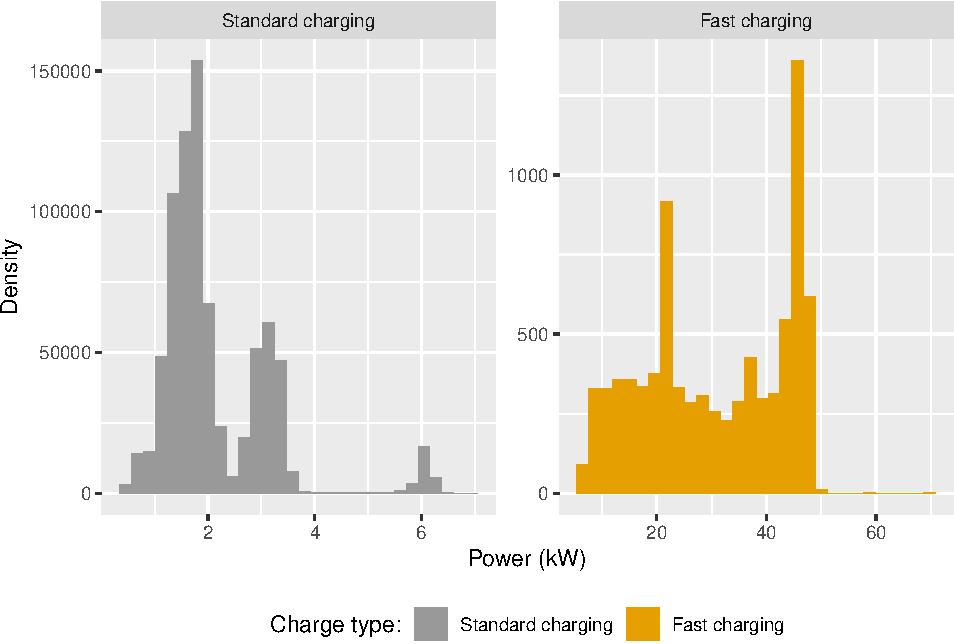
\includegraphics{EVBB_report_files/figure-latex/obsPower-1.pdf}
\caption{\label{fig:obsPower}Observed power demand distribution by day of
the week and charge type where charging observed}
\end{figure}

75\% of standard charging observations were 1.47 kW or more but the
figure was 20.28 kW or more for fast charging

\section{Daily demand}\label{daily-demand}

\begin{figure}
\centering
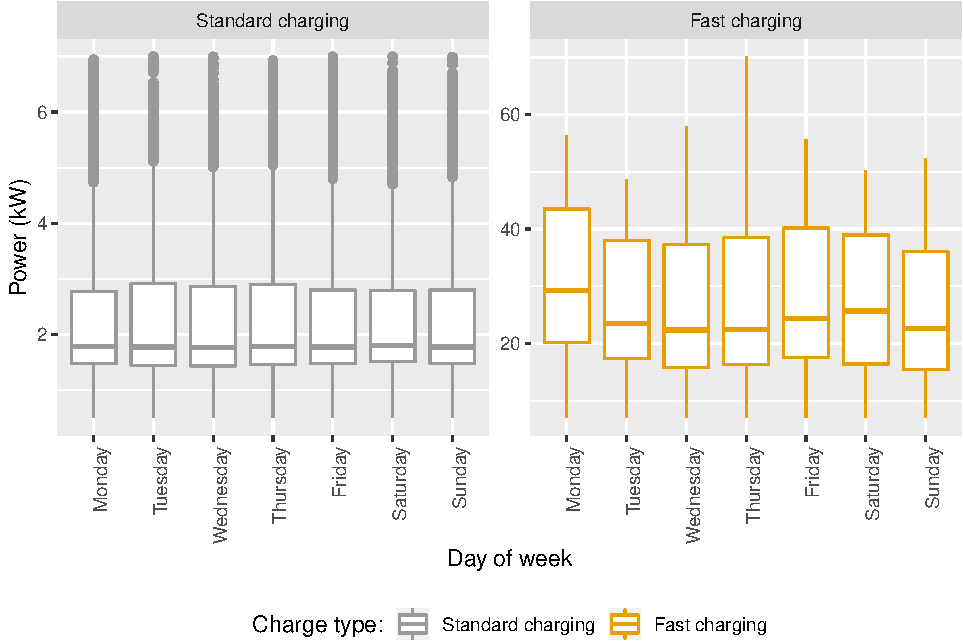
\includegraphics{EVBB_report_files/figure-latex/dailyPower-1.pdf}
\caption{\label{fig:dailyPower}Observed power demand distribution by day of
the week and charge type}
\end{figure}

Figure \ref{fig:dailyPower} shows the distribution of observed charging
kW demand by day of the week. We can see that fast charging varies in
demand more than standard charging does across days.

\section{Charging duration}\label{duration}

\section{Duration by time of day}\label{duration-by-time-of-day}

\begin{figure}
\centering
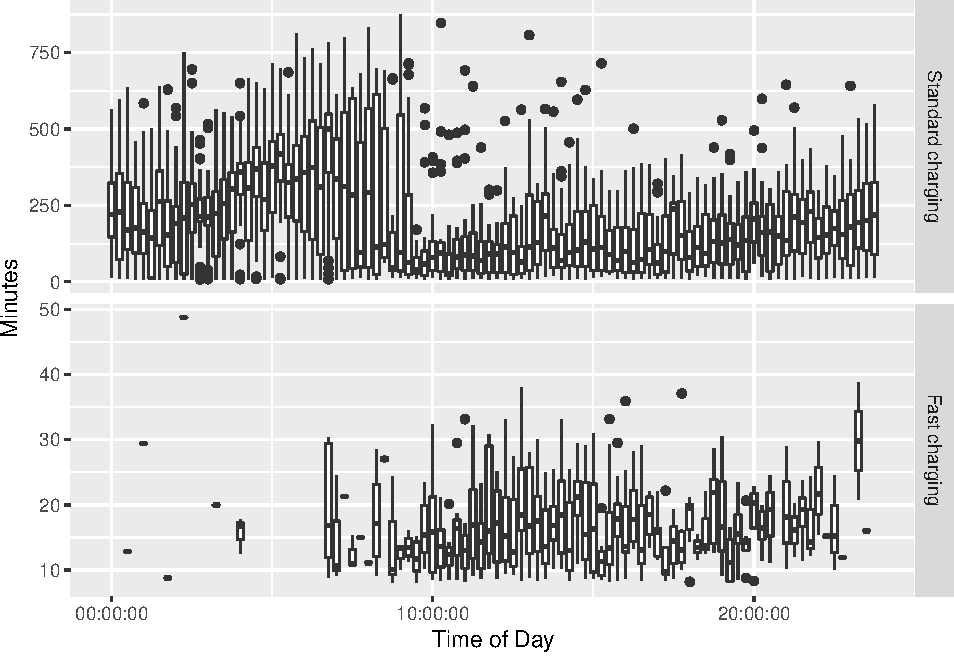
\includegraphics{EVBB_report_files/figure-latex/durationTimeBox-1.pdf}
\caption{\label{fig:durationTimeBox}Duration by time of charging start}
\end{figure}

\begin{figure}
\centering
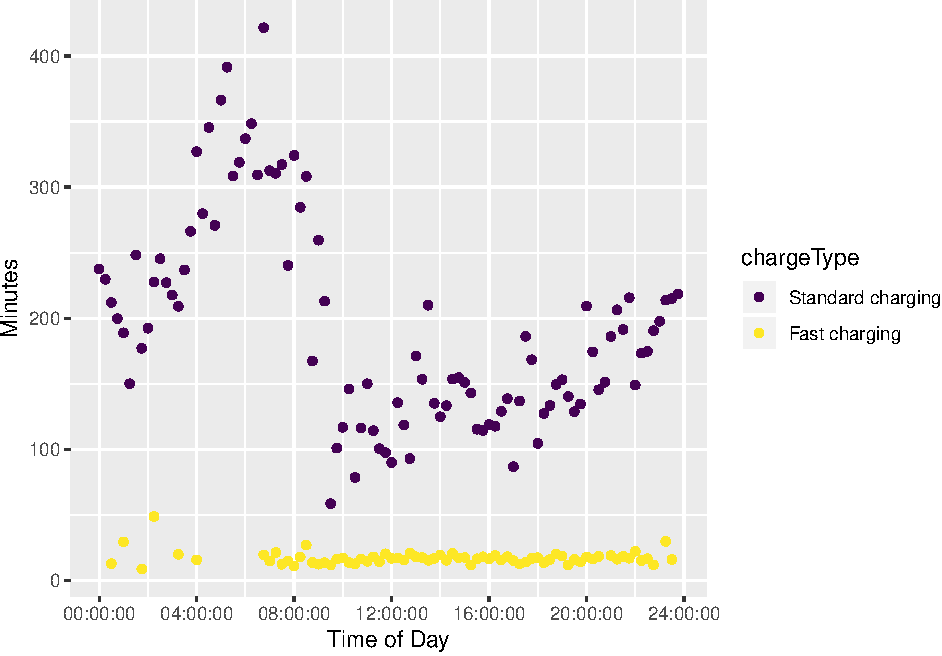
\includegraphics{EVBB_report_files/figure-latex/durationTimeMean-1.pdf}
\caption{\label{fig:durationTimeMean}Mean duration (within quarter hours) by
time of charging start for sequences \textgreater{} 8 minutes}
\end{figure}

\begin{table}[t]

\caption{\label{tab:meanDurationTable}Mean duration of charge events by charge type}
\centering
\begin{tabular}{l|r|r|r|r|r}
\hline
chargeType & N & mean & median & min & max\\
\hline
Standard charging & 2860 & 244.00682 & 208.65000 & 8.016667 & 1616.717\\
\hline
Fast charging & 279 & 51.61231 & 15.73333 & 8.050000 & 8621.000\\
\hline
\end{tabular}
\end{table}

\section{Time of charging}\label{time-of-charging}

\begin{figure}
\centering
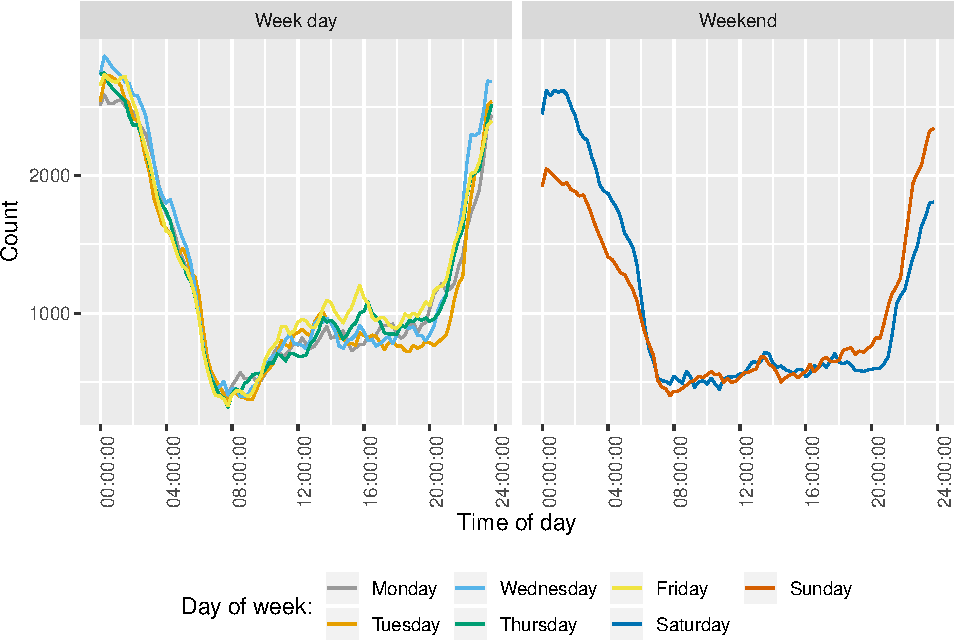
\includegraphics{EVBB_report_files/figure-latex/chargeTime-1.pdf}
\caption{\label{fig:chargeTime}Count of observed charging events by type,
day of week and time}
\end{figure}

Figure \ref{fig:chargeTime} shows the distribution of observed charging
by time of day and day of the week. Aggregating counts in this way
emphasises the times at which charging most commonly occurs and we can
see\ldots{}

Fig: profile of median charging demand by time of day and day of the
week faceted by at home vs not at home

Charging demand varies somewhat by time of day and day of the week.
Weekdays show \ldots{} whilst weekends show. Saturdays and Sundays vary
with\ldots{}

\begin{figure}
\centering
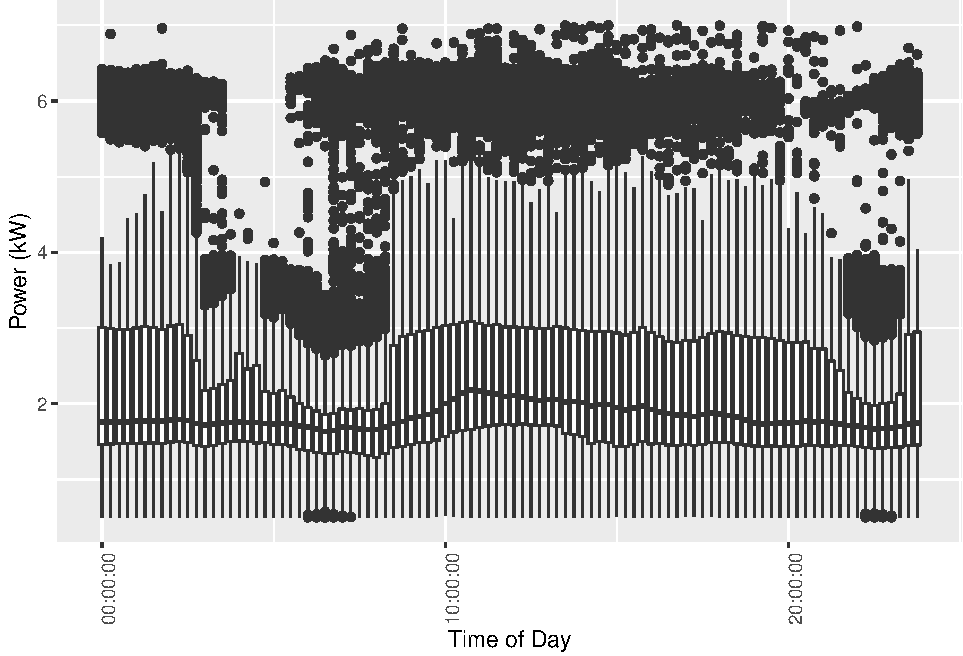
\includegraphics{EVBB_report_files/figure-latex/boxplotCharging-1.pdf}
\caption{\label{fig:boxplotCharging}Boxplot of charging timing by charge
rate}
\end{figure}

\begin{figure}
\centering
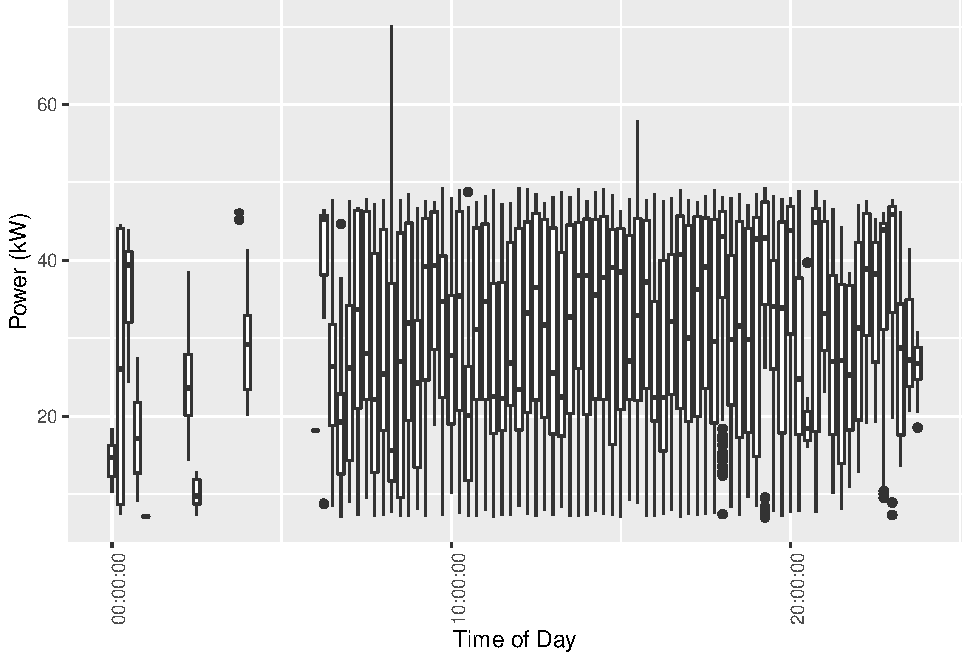
\includegraphics{EVBB_report_files/figure-latex/plot3-1.pdf}
\caption{\label{fig:plot3}Boxplot of charging timing by charge rate}
\end{figure}

\begin{figure}
\centering
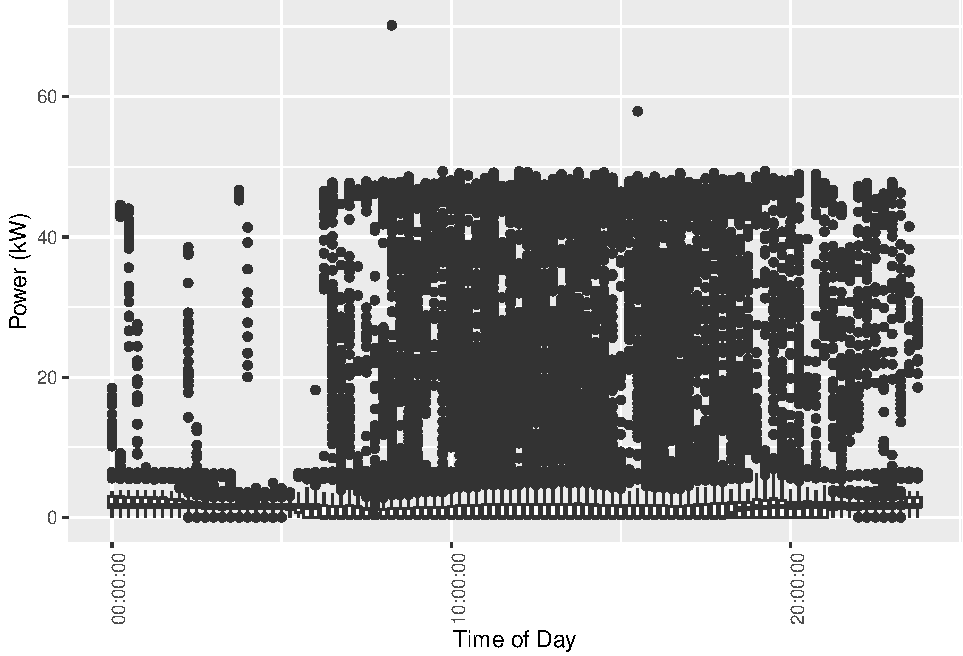
\includegraphics{EVBB_report_files/figure-latex/plot2-1.pdf}
\caption{\label{fig:plot2}Boxplot of charging timing}
\end{figure}

\begin{verbatim}
## Picking joint bandwidth of 5860
\end{verbatim}

\begin{figure}
\centering
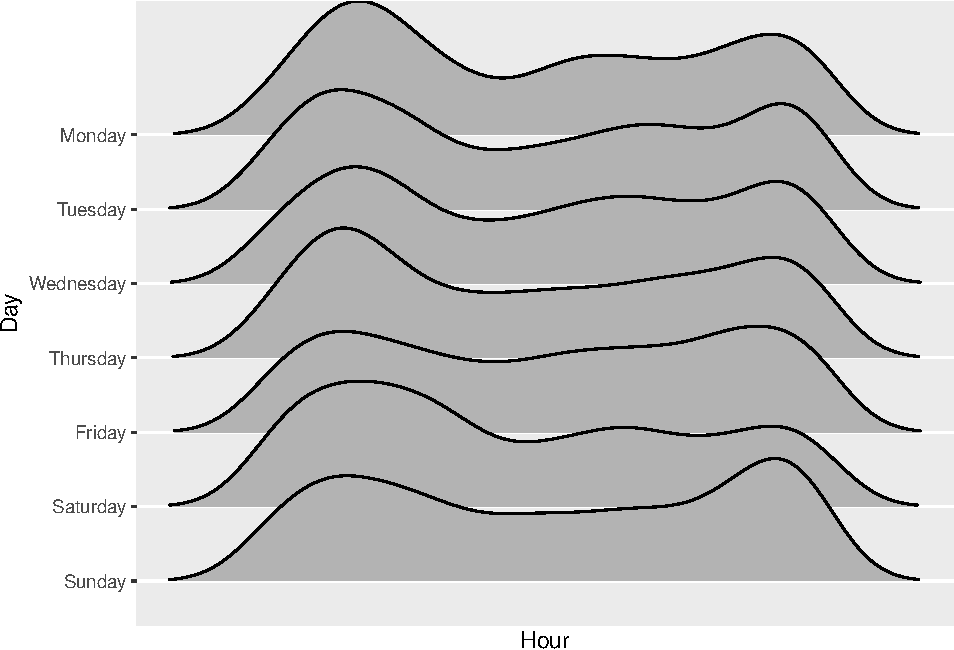
\includegraphics{EVBB_report_files/figure-latex/ggjoyplotTimeChargingBegins-1.pdf}
\caption{\label{fig:ggjoyplotTimeChargingBegins}Time charging begins}
\end{figure}

\begin{verbatim}
## <ggproto object: Class FacetGrid, Facet, gg>
##     compute_layout: function
##     draw_back: function
##     draw_front: function
##     draw_labels: function
##     draw_panels: function
##     finish_data: function
##     init_scales: function
##     map_data: function
##     params: list
##     setup_data: function
##     setup_params: function
##     shrink: TRUE
##     train_scales: function
##     vars: function
##     super:  <ggproto object: Class FacetGrid, Facet, gg>
\end{verbatim}

\begin{figure}
\centering
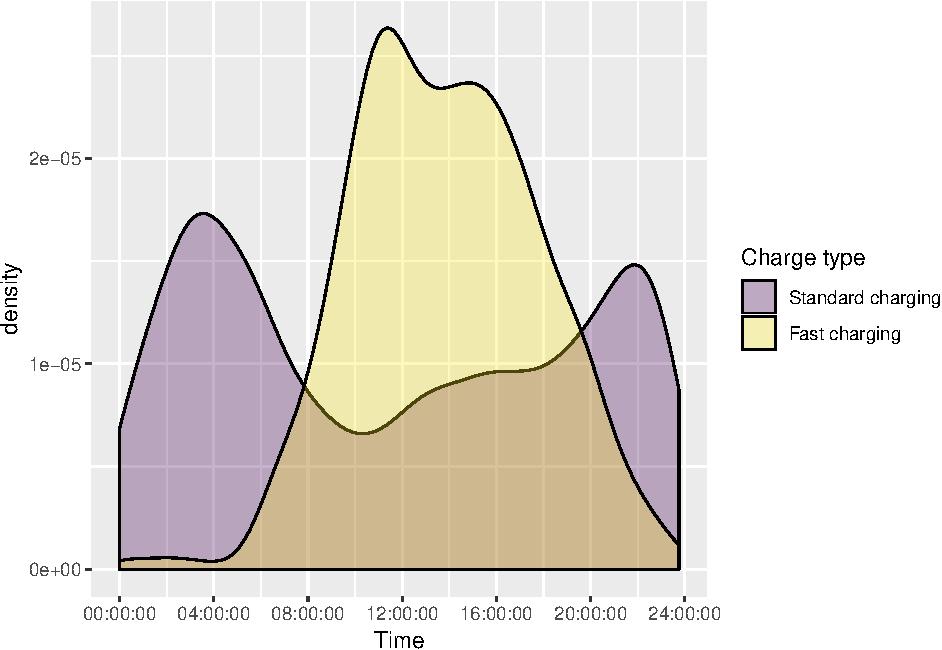
\includegraphics{EVBB_report_files/figure-latex/chargeBeginsWeekday-1.pdf}
\caption{\label{fig:chargeBeginsWeekday}Density plot of charging start times
during weekdays}
\end{figure}

\begin{figure}
\centering
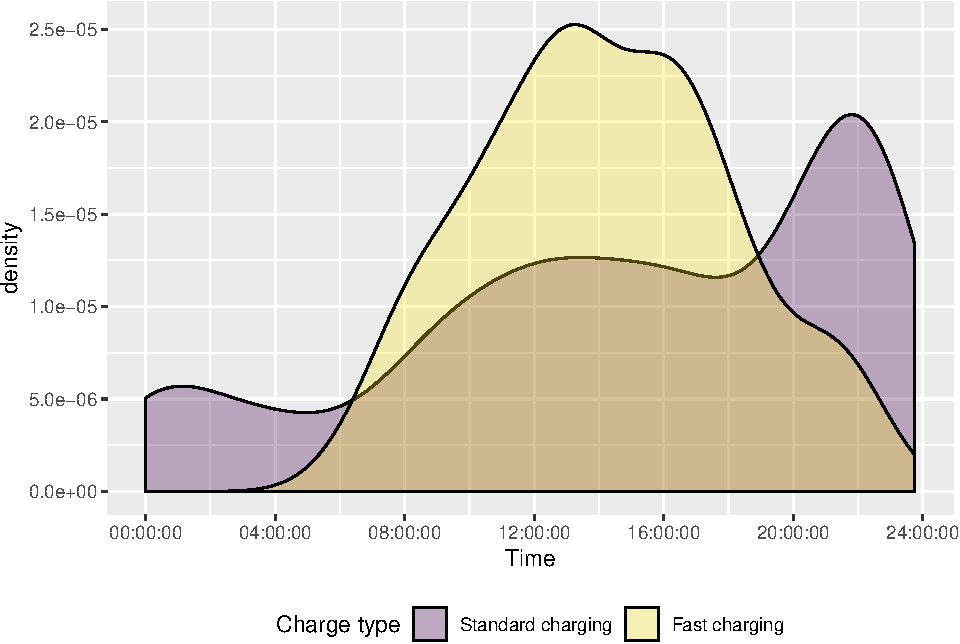
\includegraphics{EVBB_report_files/figure-latex/chargeBeginsWeekend-1.pdf}
\caption{\label{fig:chargeBeginsWeekend}Density plot of charging start times
during weekends}
\end{figure}

\begin{figure}
\centering
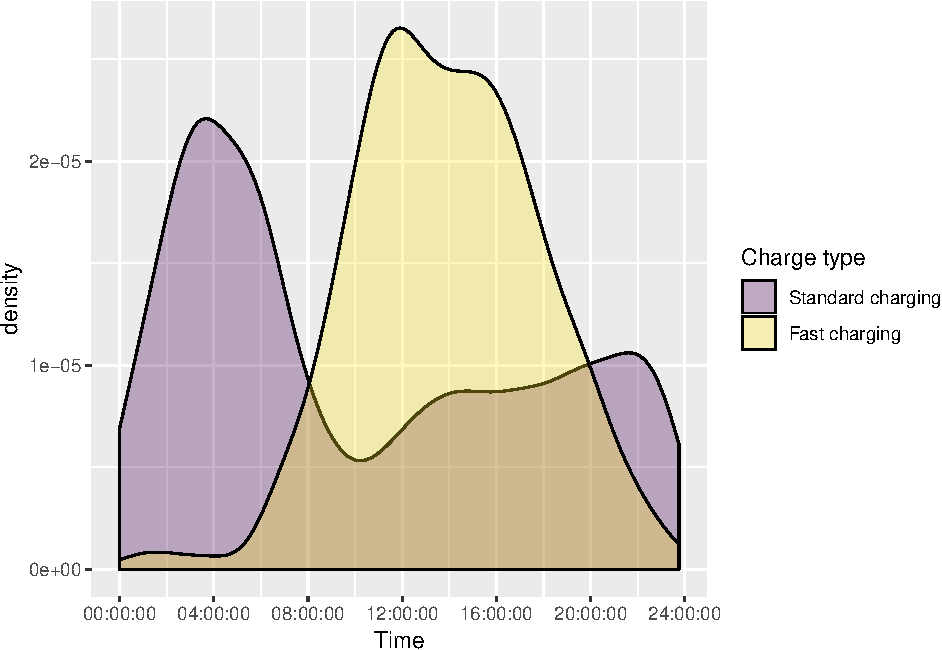
\includegraphics{EVBB_report_files/figure-latex/chargeEndsWeekday-1.pdf}
\caption{\label{fig:chargeEndsWeekday}Density plot of charging end times
during weekdays}
\end{figure}

\begin{figure}
\centering
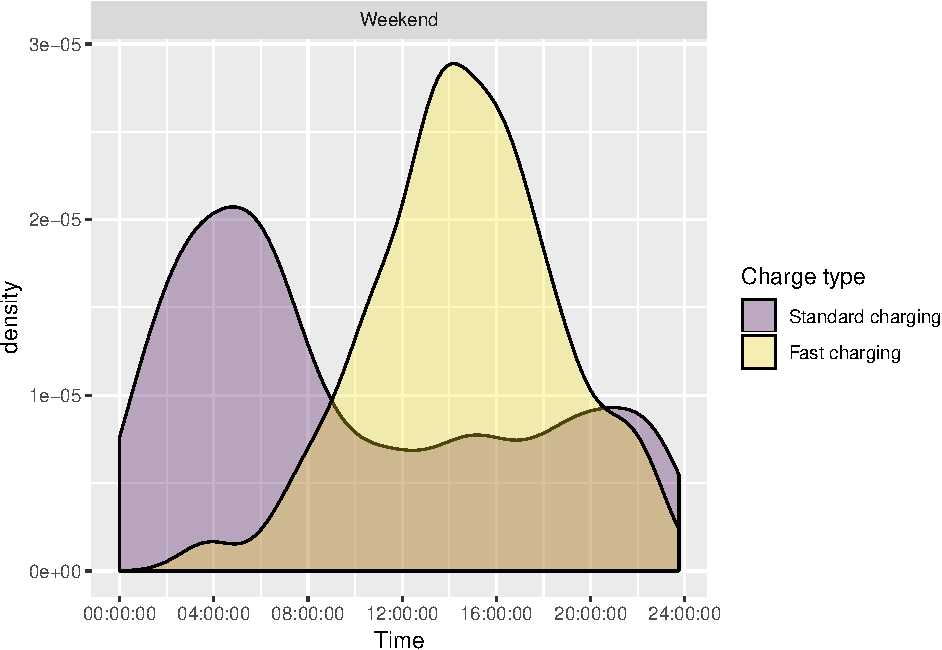
\includegraphics{EVBB_report_files/figure-latex/chargeEndsWeekend-1.pdf}
\caption{\label{fig:chargeEndsWeekend}Density plot of charging end times
during weekends}
\end{figure}

At home charging events tended to begin at HH:MM during weekdays and
HH:MM at weekends. \emph{We can get ``Slow'' charging events rather than
``home''}

Standard charging has a noticeably different profile to charging
patterns for fast charges. It suggests that it is common for plug-in
vehicle owners to charge overnight at home, and perhaps use the more
powerful public chargepoints to top up during the day.

\begin{quote}
Discuss any other patterns
\end{quote}

\section{State of charge}\label{state-of-charge}

The duration of charging events (see Section \ref{duration}) suggests
that EVs may be `plugged in' at home (and elsewhere) for considerable
durations.

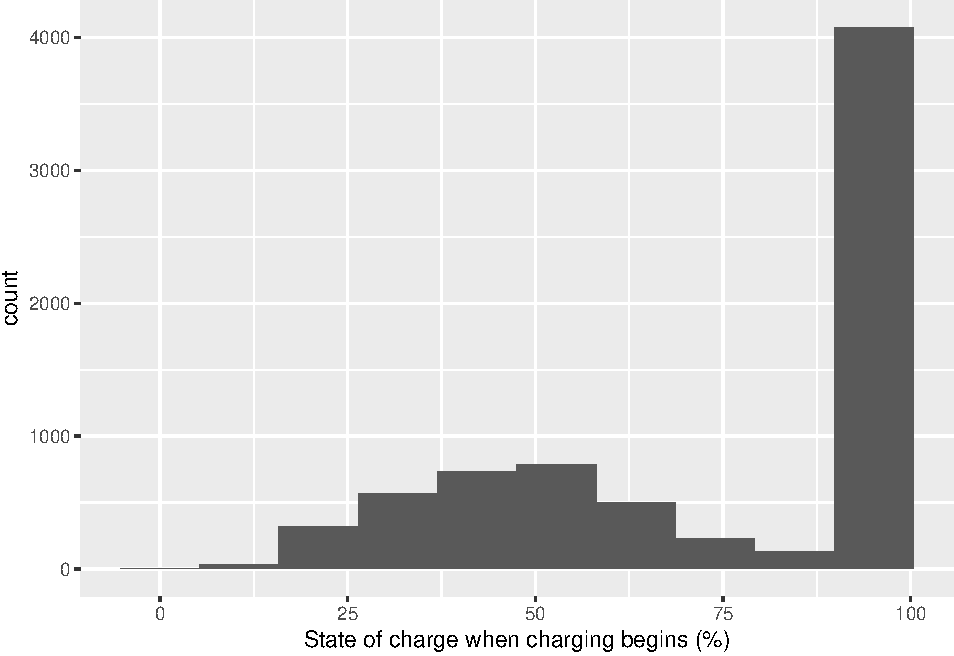
\includegraphics{EVBB_report_files/figure-latex/value of state of charge at beginning of charge-1.pdf}

\begin{verbatim}
## Saving 6.5 x 4.5 in image
\end{verbatim}

Fig: Distribution of state of charge when evening charge event starts
`at home' (histogram (or joy plot) by day of week)
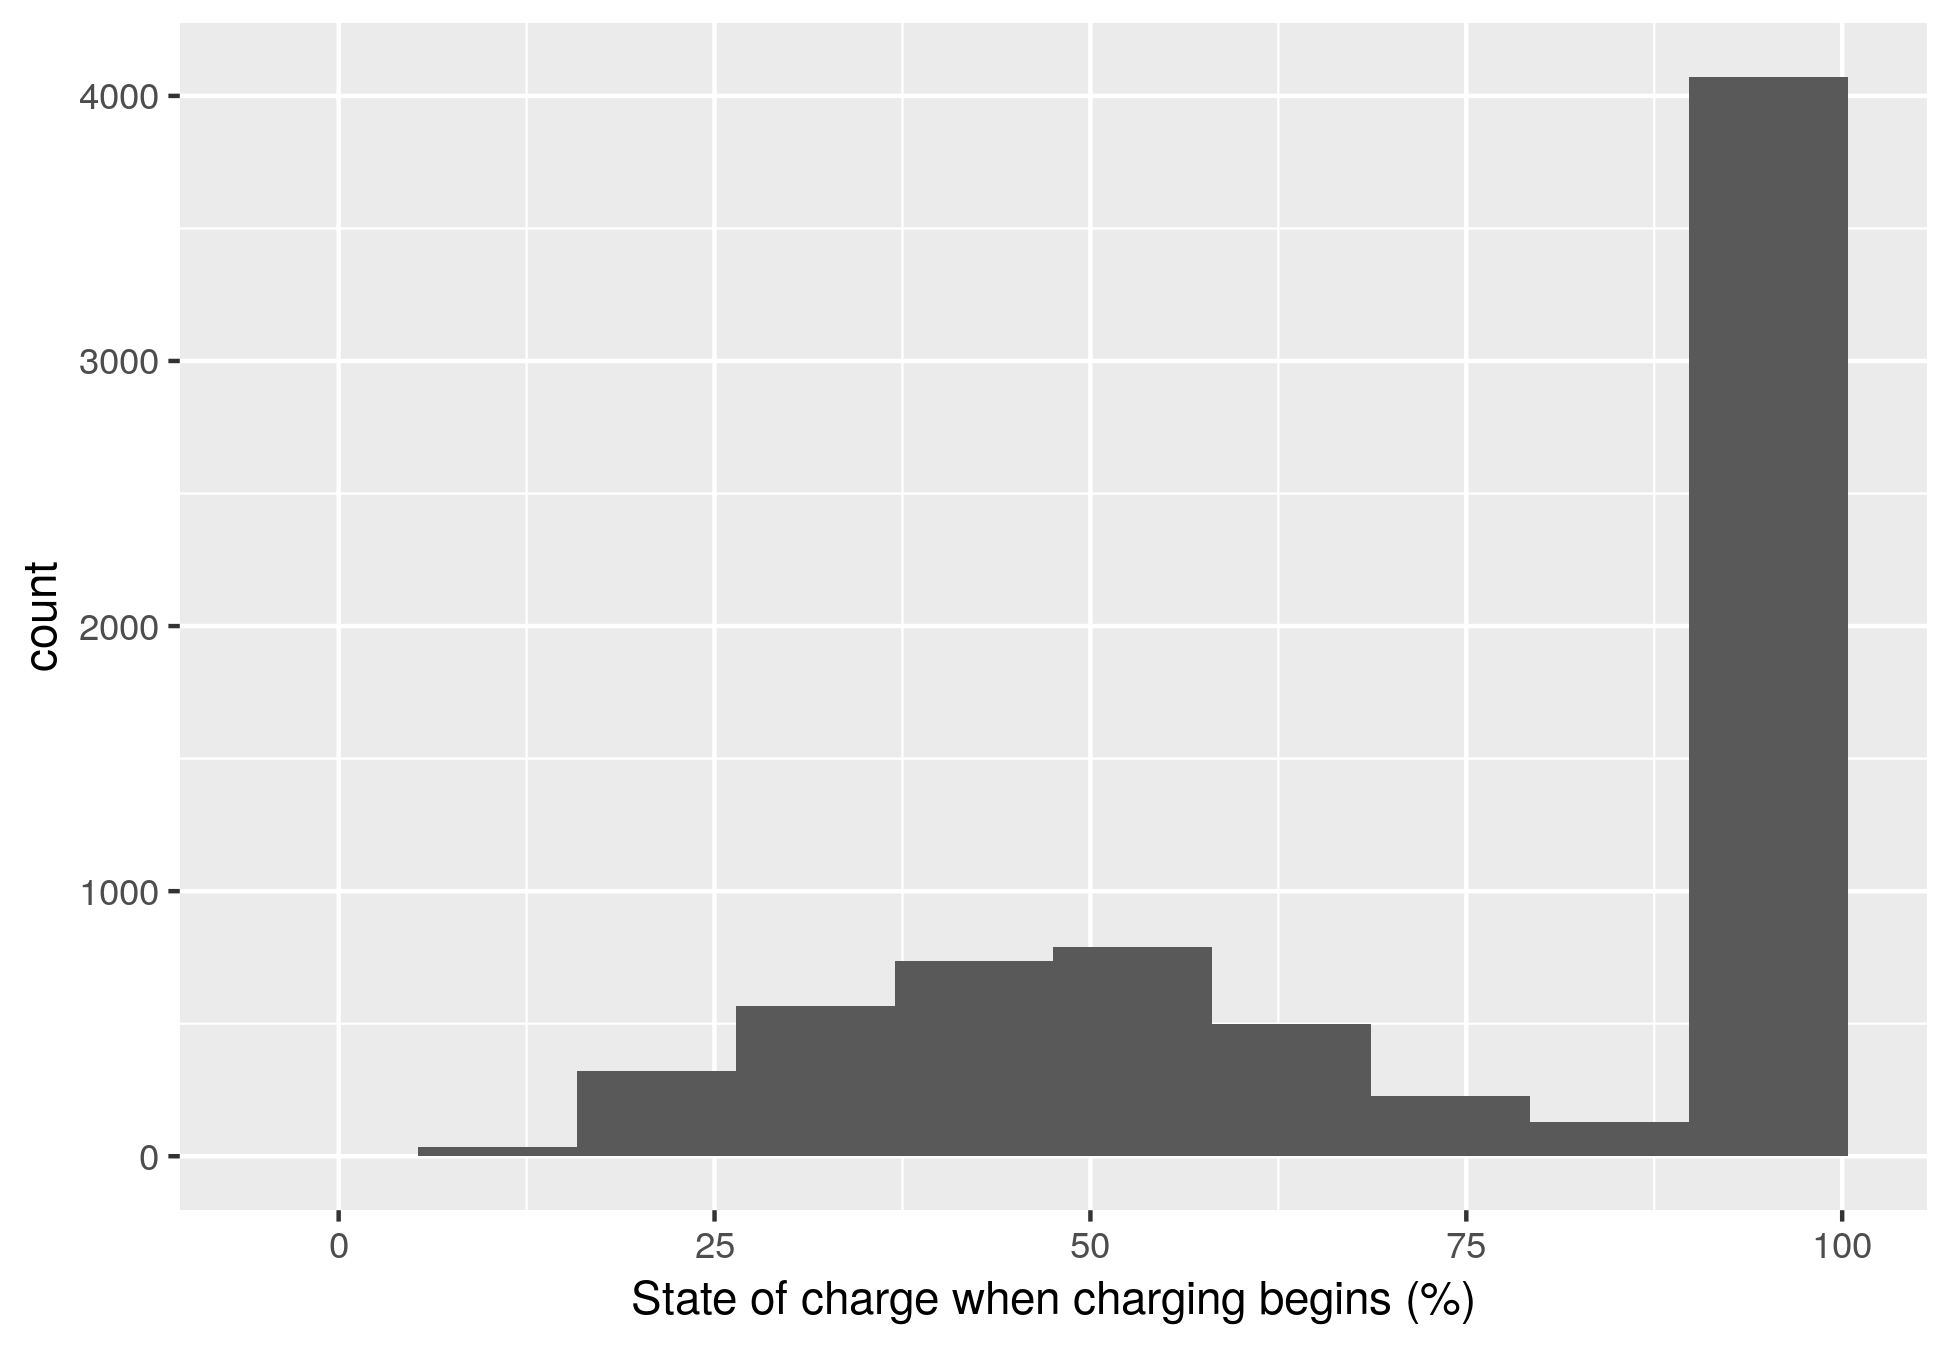
\includegraphics{~/EVBB/plots/SOC_when_charging_begins.png}

The figure shows that many vehicles arrive home with greater than 50\%
charge remaining and would therefore be able to transfer energy to the
home during the evening grid peak as a form of demand response.

Fig: Mean state of battery charge at the first `at home' charging
observation by hour and day of the week \emph{No ``at home'' data with
SOC}

\begin{quote}
should show the timing of `coming home' battery state?
\end{quote}

Fig: Distribution of duration of charge events starting `at home' in the
evening (by day of the week) \emph{Duration difficult to accurately
determine without date due to charging occurring through the night}

The figure shows that vehicles may then be available for further demand
response and/or re-charging for up to XX hours from this point.

\begin{quote}
Discuss any other patterns
\end{quote}


\end{document}
